% Created 2025-10-22 Wed 19:32
% Intended LaTeX compiler: pdflatex
\documentclass[smaller,aspectratio=169]{beamer}
\usepackage[utf8]{inputenc}
\usepackage[T1]{fontenc}
\usepackage{graphicx}
\usepackage{longtable}
\usepackage{wrapfig}
\usepackage{rotating}
\usepackage[normalem]{ulem}
\usepackage{amsmath}
\usepackage{amssymb}
\usepackage{capt-of}
\usepackage{hyperref}
\usepackage{minted}
\usemintedstyle{tango} \setminted{fontfamily="Mononoki Nerd Font", breaklines=true, breakanywhere=true, fontsize=\large}
\usetheme{default}
\usecolortheme{wolverine}
\author{Oliver Pauffley}
\date{\today}
\title{Nix for Reproducible Developer Environments}
\beamerdefaultoverlayspecification{<+->}
\hypersetup{
 pdfauthor={Oliver Pauffley},
 pdftitle={Nix for Reproducible Developer Environments},
 pdfkeywords={},
 pdfsubject={},
 pdfcreator={Emacs 30.2 (Org mode 9.7.34)}, 
 pdflang={English}}
\begin{document}

\maketitle
\begin{frame}[label={sec:org0ea4ea8}]{Protobuf}
\begin{center}
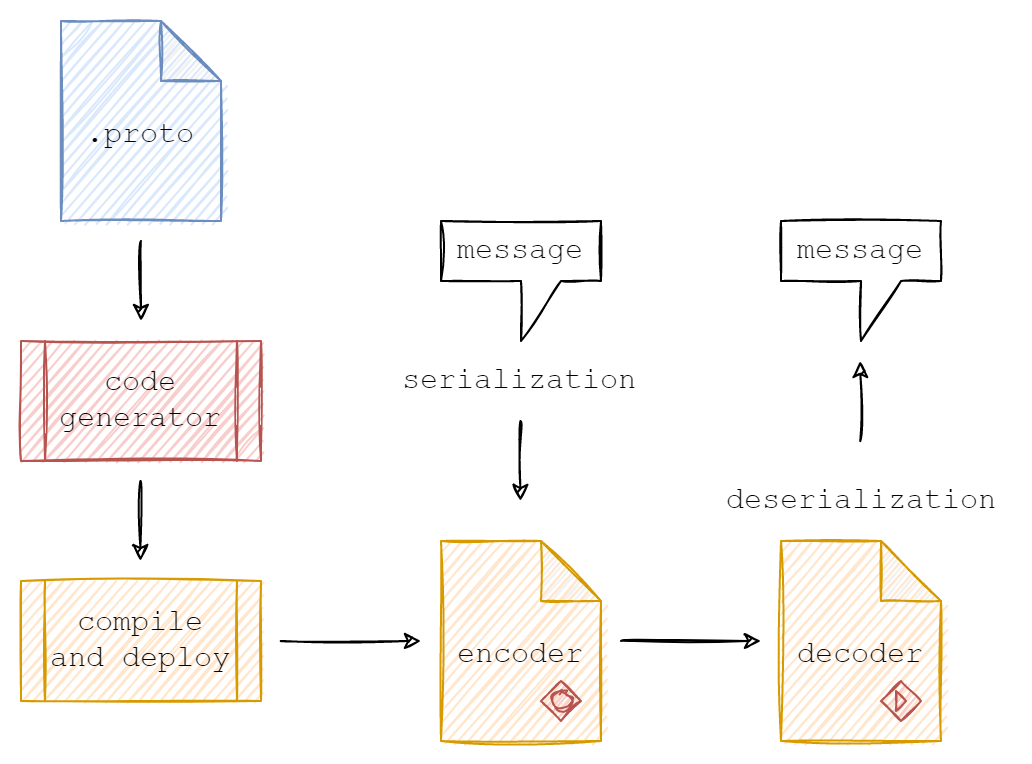
\includegraphics[width=250px]{./what_are_protos.png}
\end{center}
\end{frame}
\begin{frame}[label={sec:org413fbe6}]{Version Number Wars}
\begin{columns}
\begin{column}[t]{0.45\columnwidth}
Everyone loves a PR with 2000+ changes.
\begin{center}

\includegraphics[width=.9\linewidth]{./pr_size.png}
\end{center}
\end{column}
\begin{column}[t]{0.45\columnwidth}
But drilling down.
\begin{center}
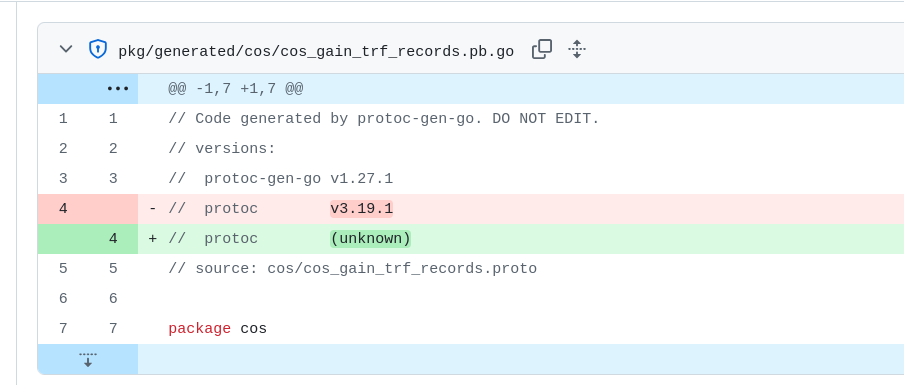
\includegraphics[width=.9\linewidth]{./why_big.png}
\end{center}
\end{column}
\end{columns}
\end{frame}
\begin{frame}[label={sec:org2cb7d8a}]{The Problem}
Every developer has a different version of the tools used to generate the protos!
\end{frame}
\begin{frame}[label={sec:orgb0d987e},fragile]{Make - Install everything on my machine}
 Lets just include instructions on how to install things
\begin{minted}[]{makefile}
PROTOC_VERSION := 3.14.0
.PHONY: install-protoc
install-protoc:
	curl -OL https://github.com/protocolbuffers/protobuf/releases/download/v$(PROTOC_VERSION)/$(PROTOC_FILE)
	sudo unzip -o $(PROTOC_FILE) -d /usr/local bin/protoc
	sudo unzip -o $(PROTOC_FILE) -d /usr/local 'include/*'
	rm -f $(PROTOC_FILE)
\end{minted}
\end{frame}
\begin{frame}[label={sec:org3cd18a6}]{Ahh?}
\begin{itemize}
\item Turns out this was already in the repo.
\item I don't really want to have curl installing things.
\item You can just ignore it.
\end{itemize}
\end{frame}
\begin{frame}[label={sec:orgdf6cf9e}]{Install everything on someone else's machine}
\begin{itemize}
\item If only there was a way to build a little mini machine with the binaries I need already on it.
\item Distribute the machine.
\item Docker!
\end{itemize}
\end{frame}
\begin{frame}[label={sec:org1481ca3},fragile]{Docker}
 \begin{minted}[]{dockerfile}
FROM cimg/go:1.19-node as build-stage

ENV PROTOC_VERSION=3.18.1

# Install protoc
RUN curl -LO https://github.com/protocolbuffers/protobuf/releases/download/v${PROTOC_VERSION}/protoc-${PROTOC_VERSION}-linux-x86_64.zip
RUN unzip protoc-${PROTOC_VERSION}-linux-x86_64.zip -d $HOME/.local
RUN rm protoc-${PROTOC_VERSION}-linux-x86_64.zip

RUN mkdir -p /home/circleci/project/pkg/generated

# Install go/js tooling
ADD Makefile .
ADD go.mod .
ADD go.sum .
ADD package.json .
ADD yarn.lock .
RUN make install

ADD . .
# Generate code from proto files.
RUN make protos-generate

FROM scratch as export-stage

COPY --from=build-stage /home/circleci/project/pkg/generated /pkg/generated
\end{minted}
\end{frame}
\begin{frame}[label={sec:org6152165},fragile]{Docker}
 \begin{columns}
\begin{column}[t]{0.45\columnwidth}
Pros:
\begin{itemize}
\item We can distribute this file and get the same(ish) system for everyone
\item We can use it CI/CD
\end{itemize}
\end{column}
\begin{column}[t]{0.45\columnwidth}
Cons:
\begin{itemize}
\item We have actually only lifted the problem into docker
\item \texttt{ADD package.json}
\item This is only as deterministic as the package management we are using within docker.
\item Very slow
\item Doesn't connect well with local tooling for devs
\end{itemize}
\end{column}
\end{columns}
\end{frame}
\begin{frame}[label={sec:org48324c1}]{Nix - Install everything on my machine the same as everyone else's}
\end{frame}
\begin{frame}[label={sec:org85fe781}]{Demo}
\end{frame}
\begin{frame}[label={sec:org46532f6}]{Is Nix for You?}
\begin{columns}
\begin{column}{0.45\columnwidth}
Almost definitely no\ldots{}
\begin{itemize}
\item It's a little complicated to learn (But really not a big barrier to entry).
\item The payoff is complicated to explain.
\item Error messages are difficult to understand.
\end{itemize}
But
\begin{itemize}
\item It's probably the future?
\item When it's working and setup it's incredibly powerful.
\item You are probably rebuilding it's features yourself.
\end{itemize}
\end{column}
\begin{column}{0.45\columnwidth}
\begin{quote}
I’ve been a happy Nix user for about 18 months now, and– well, not happy happy, but satisfied… no… not really satisfied either; perhaps it’s more of a resigned disgruntlement; a feeling that despite its many flaws, it’s still better than anything else out there, and I’ve invested so much time into it already that it would be a shame to give up now, so… am I describing Stockholm syndrome?
--- Ian Henry
\end{quote}
\end{column}
\end{columns}
\end{frame}
\begin{frame}[label={sec:orgd4c0726}]{How to install Nix}
\url{https://nixos.org/download/}

\begin{itemize}
\item Works on linux, mac and windows (through wsl)
\item You can use it as well as your other package managers
\end{itemize}
\end{frame}
\begin{frame}[label={sec:org1095588}]{Haskell Book Club}
I also run a monthly haskell book club. Meeting on the last Sunday of the month
\end{frame}
\begin{frame}[label={sec:orgc03cf00}]{Questions?}
\end{frame}
\end{document}
